%************************************************
\section{算法、代码、表格、图片和引用}
\begin{frame}[fragile]\frametitle{插入算法v1.0}
  \begin{columns}
    \begin{column}{0.05\textwidth}
    \end{column}
    \begin{column}{0.45\textwidth}
    \begin{block}{Input}
    \begin{verbatim}
\begin{algorithm}[H]
\caption{An Algorithm}
\begin{algorithmic}[1]
\FOR{each $i in [1,9]$}
\STATE initialize $T_{i}$;\
\STATE $T_{i};$\
\ENDFOR
\end{algorithmic}
\end{algorithm}
    \end{verbatim}
    \end{block}
    \end{column}
    \begin{column}{0.025\textwidth}
    \end{column}
    \begin{column}{0.45\textwidth}
    \begin{block}{Output}
\begin{algorithm}[H]
\caption{An Algorithm}
\begin{algorithmic}[1]
\FOR{each $i in [1,9]$}
\STATE initialize $T_{i}$;\
\STATE $T_{i};$\
\ENDFOR
\end{algorithmic}
\end{algorithm}
    \end{block}
    \end{column}
    \begin{column}{0.025\textwidth}
    \end{column}
  \end{columns}
\end{frame}

\begin{frame}[fragile]\frametitle{插入算法v2.0}
  \begin{columns}
    \begin{column}{0.05\textwidth}
    \end{column}
    \begin{column}{0.45\textwidth}
    \begin{block}{Input}
    \begin{verbatim}
\begin{algorithm}[H]
\caption{Description}
\begin{algorithmic}[1]
\REQUIRE ~~\\
The samples, $P_n$;\\
\ENSURE ~~\\
Classifiers, $E_n$;\\
\STATE Samples $T_n$;
\STATE Classifiers $E$
\end{algorithmic}
\end{algorithm}
    \end{verbatim}
    \end{block}
    \end{column}
    \begin{column}{0.025\textwidth}
    \end{column}
    \begin{column}{0.45\textwidth}
    \begin{block}{Output}
\begin{algorithm}[H]
\caption{Description}
\begin{algorithmic}[1]
\REQUIRE ~~\\
The samples, $P_n$;\\
\ENSURE ~~\\
Classifiers, $E_n$;\\
\STATE Samples $T_n$;
\STATE Classifiers $E$
\end{algorithmic}
\end{algorithm}
    \end{block}
    \end{column}
    \begin{column}{0.025\textwidth}
    \end{column}
  \end{columns}
\end{frame}

\begin{frame}[fragile]\frametitle{插入代码v1.0}
  \begin{columns}
    \begin{column}{0.05\textwidth}
    \end{column}
    \begin{column}{0.45\textwidth}
    \begin{block}{Input}
    \begin{verbatim}
\usepackage{listings}
\begin{lstlisting}
[language=C]
int main(void)
{
printf("Hello world!\n");
return 0;
}
\end{lstlisting}
    \end{verbatim}
    \end{block}
    \end{column}
    \begin{column}{0.025\textwidth}
    \end{column}
    \begin{column}{0.45\textwidth}
\begin{lstlisting}[language=C]
int main(void)
{
printf("Hello world!\n");
return 0;
}
\end{lstlisting}
    \end{column}
    \begin{column}{0.025\textwidth}
    \end{column}
  \end{columns}
\end{frame}

\begin{frame}[fragile]\frametitle{插入代码v6.0}
  \begin{columns}
    \begin{column}{0.005\textwidth}
    \end{column}
    \begin{column}{0.425\textwidth}
    \begin{block}{Input}
    \begin{verbatim}
\lstset
{numbers=left,blarblar}
\begin{lstlisting}
[language=C]
int main(void)
{
printf("Hello world!\n");
return 0;
}
\end{lstlisting}
    \end{verbatim}
    \end{block}
    \end{column}
    \begin{column}{0.025\textwidth}
    \end{column}
    \begin{column}{0.52\textwidth}
\begin{lstlisting}[language=C, numbers=left,
numberstyle=\tiny, keywordstyle=\color{blue!70}, commentstyle=\color{red!50!green!50!blue!50},
frame=shadowbox, rulesepcolor=\color{red!20!green!20!blue!20}]
int main(void)
{
/* print a string*/
printf("Hello world!\n");
return 0;
}
\end{lstlisting}
    \end{column}
    \begin{column}{0.025\textwidth}
    \end{column}
  \end{columns}
\end{frame}

\begin{frame}[fragile]\frametitle{插入表格}
  \begin{columns}
    \begin{column}{0.05\textwidth}
    \end{column}
    \begin{column}{0.45\textwidth}
    \begin{block}{Input}
    \begin{verbatim}
\begin{tabular}{l|l}
Name & score \\
\hline
You & 100 \\
Me & 59
\end{tabular}
    \end{verbatim}
    \end{block}
    \end{column}
    \begin{column}{0.05\textwidth}
    \end{column}
    \begin{column}{0.40\textwidth}
    \begin{block}{Output}
        \begin{tabular}{l|l}
        Name & score \\
        \hline
        You & 100 \\
        Me & 59
        \end{tabular}
    \end{block}
    \end{column}
    \begin{column}{0.05\textwidth}
    \end{column}
  \end{columns}
\end{frame}

\begin{frame}[fragile]\frametitle{图片格式支持什么?}
    \begin{description}
		\item[ps]: PostScript. 由Adobe公司推出,是一种页面描述语言。独立于设备,能综合处理文字和图像,擅长于描述矢量图形。
		\item[eps]: Encapsulated PostScript. 封装的PostScript,是PostScript的一个子集,每个eps文件只有一个页面。eps格式的图片与\LaTeX 最兼容。
        \item[pdf]: Portable Document Format
		\item[非矢量图]:jpg, png, bmp, \ldots : 各种其他图片格式,也被\LaTeX 支持
	\end{description}
\end{frame}

\begin{frame}[fragile]\frametitle{插入jpg图片}
   \begin{block}{Input}
    \begin{verbatim}
\begin{figure}[h]
    \centering
    \includegraphics[width=0.3\textwidth,angle=20]{jpg_figure}
\end{figure}
    \end{verbatim}
   \end{block}
   \begin{figure}[h]
    \centering
    \includegraphics[width=0.3\textwidth,angle=20]{jpg_figure}
   \end{figure}
\end{frame}

%看源码的同学,这里我要说明下,本来想做个eps的例子,但是由于这个beamer是pdflatex编译的(最初2了)
%如果要编译eps,需要用latex 或 xelatex
\begin{frame}[fragile]\frametitle{矢量图vs非矢量图}
    \begin{center}
    \includegraphics[height=0.3\textwidth]{eps_figure.eps}\qquad
    \includegraphics[height=0.3\textwidth]{png_figure.png}
    \end{center}
\end{frame}


\begin{frame}[fragile]\frametitle{插入eps图片}
   \begin{block}{Input}
    \begin{verbatim}
    \includegraphics[width=0.5\textwidth]{eps_figure.eps}
    \end{verbatim}
   \end{block}
   \begin{figure}[h]
    \centering
    \includegraphics[width=0.5\textwidth]{eps_figure.eps}
   \end{figure}
\end{frame}

\begin{frame}[fragile]\frametitle{插入pdf图片}
   \begin{block}{Input}
    \begin{verbatim}
    \includegraphics[width=0.5\textwidth]{pdf_figure.pdf}
    \end{verbatim}
   \end{block}
   \begin{figure}[h]
    \centering
    \includegraphics[width=0.5\textwidth]{pdf_figure.pdf}
   \end{figure}
\end{frame}

\begin{frame}\frametitle{插入MetaPost}
   \begin{figure}[h]
    \centering
    \includegraphics[width=1\textwidth]{metapost_figure}
   \end{figure}
\end{frame}

\begin{frame}\frametitle{插入TikZ}
   \begin{figure}\setcounter{subfigure}{0}
    \centering
    \subfigure[$G$~(无向图)]{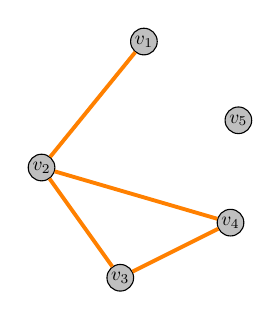
\begin{tikzpicture}
    \tikzstyle{every node}=[inner sep=1pt,circle,draw,fill=black!25,scale=0.7]
    \path (0,0) node(3) {$v_3$}
          (-1,1.4) node(2) {$v_2$}
          (0.3,3) node(1) {$v_1$}
          (1.4,0.7) node(4) {$v_4$}
          (1.5,2) node(5) {$v_5$};
    \foreach \source/\target in {1/2, 2/3, 3/4, 4/2}
    \draw[orange,line width=1.4pt] (\source) --(\target);
    \end{tikzpicture}}\qquad
    \subfigure[$G'$~(有向图)]{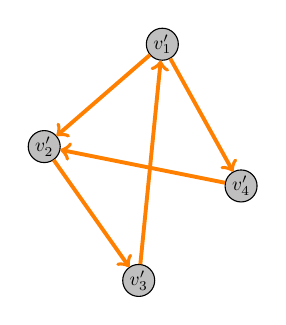
\begin{tikzpicture}
    \tikzstyle{every node}=[inner sep=1pt,circle,draw,fill=black!25,scale=0.7]
    \path (0,0) node(3) {$v_3'$}
          (-1.2,1.7) node(2) {$v_2'$}
          (0.3,3) node(1) {$v_1'$}
          (1.3,1.2) node(4) {$v_4'$};
    \foreach \source/\target in {1/2, 2/3, 3/1, 4/2, 1/4}
    \draw[->,orange,line width=1.4pt] (\source) --(\target);
    \end{tikzpicture}}\qquad
    \subfigure[$G''$~(混合图)]{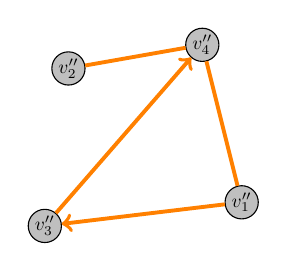
\begin{tikzpicture}
    \tikzstyle{every node}=[inner sep=1pt,circle,draw,fill=black!25,scale=0.7]
    \path (0,0) node(3) {$v_3''$}
          (0.3,2) node(2) {$v_2''$}
          (2.5,0.3) node(1) {$v_1''$}
          (2,2.3) node(4) {$v_4''$};
    \foreach \source/\target in {1/3, 3/4}
    \draw[->,orange,line width=1.4pt] (\source) --(\target);
    \draw[orange,line width=1.4pt] (2) --(4);
    \draw[orange,line width=1.4pt] (1) --(4);
    \end{tikzpicture}}
    \end{figure}
\end{frame}


\begin{frame}[fragile]\frametitle{引用}
  \begin{columns}
    \begin{column}{0.01\textwidth}
    \end{column}
    \begin{column}{0.55\textwidth}
    \begin{block}{Input}
    \begin{verbatim}
\begin{equation}
\lim_{x \to 0}\frac{\sin x}{x}=1
\label{myequation}
\end{equation}
(\ref{myequation})式是一个很重要的极限
    \end{verbatim}
    \end{block}
    \end{column}
    \begin{column}{0.025\textwidth}
    \end{column}
    \begin{column}{0.4\textwidth}
    \begin{block}{Output}
        \begin{equation}
        \lim_{x \to 0}\frac{\sin x}{x}=1
        \label{myequation}
        \end{equation}
        (\ref{myequation})式是一个很重要的极限
    \end{block}
    \end{column}
    \begin{column}{0.015\textwidth}
    \end{column}
  \end{columns}
\end{frame}
